%==============================================================================
% Exemplo de Dissertação de mestrado com a classe texufpel
%
% Adaptação do exemplo de TCC (tcc/exemplo-tcc.tex) para dissertação. O texto
% de cada seção explica o recurso que aparece nela. As diferenças em relação
% ao TCC estão marcadas com "DISSERTAÇÃO" nos comentários: opção diss,
% programa de pós-graduação, orientadora, lista de símbolos e errata.
% Para começar o seu trabalho, copie este arquivo, troque os dados do
% preâmbulo (os comentários "ALTERE" indicam o que mudar) e substitua o texto
% dos capítulos.
%
% Compilação (a partir da pasta raiz do repositório, onde estão a classe, o
% estilo abnt.bst, o bibliografia.bib e a pasta imagens/):
%   pdflatex dissertação/exemplo-diss
%   bibtex   exemplo-diss
%   pdflatex dissertação/exemplo-diss
%   pdflatex dissertação/exemplo-diss
% No Overleaf, basta marcar dissertação/exemplo-diss.tex como documento
% principal.
%
% As páginas citadas nos comentários são as do Manual de normas UFPel para
% trabalhos acadêmicos (2023).
%==============================================================================

% Opções da classe:
%   diss  dissertação de mestrado (DISSERTAÇÃO; use tcc, tese, eq,
%         diss-proposta... para os outros tipos)
%   capa  gera a capa (obrigatória no trabalho depositado, Manual, p. 12)
\documentclass[diss,capa]{texufpel}

%------------------------------------------------------------------------------
% Pacotes usados neste exemplo. Nenhum é obrigatório: carregue só o que o seu
% trabalho usar. A classe já carrega graphicx, hyperref, natbib e caption.
%------------------------------------------------------------------------------
\usepackage{amsmath}        % equações alinhadas (align) e \eqref
\usepackage{algpseudocode}  % pseudocódigo (ambiente algorithmic)
\usepackage{listings}       % listagens de código-fonte
\usepackage{pdfcomment}     % \pdftooltip: dica com o significado da sigla

% Referência completa em nota de rodapé (\footcite). O Manual adota o sistema
% autor-data (p. 62); use este recurso só se o curso pedir.
\usepackage{bibentry}
\nobibliography*
\newcommand{\footcite}[1]{\footnote{\bibentry{#1}}}

% Palavras do pseudocódigo em português
\algrenewcommand\algorithmicrequire{\textbf{Entrada:}}
\algrenewcommand\algorithmicensure{\textbf{Saída:}}
\algrenewcommand\algorithmicfor{\textbf{para}}
\algrenewcommand\algorithmicforall{\textbf{para cada}}
\algrenewcommand\algorithmicdo{\textbf{faça}}
\algrenewcommand\algorithmicwhile{\textbf{enquanto}}
\algrenewcommand\algorithmicif{\textbf{se}}
\algrenewcommand\algorithmicthen{\textbf{então}}
\algrenewcommand\algorithmicend{\textbf{fim}}
\algrenewcommand\algorithmicreturn{\textbf{retorne}}

% Aparência das listagens de código: fonte monoespaçada pequena, linhas
% numeradas e acentos aceitos nos comentários.
\lstset{
  basicstyle=\ttfamily\footnotesize,
  numbers=left, numberstyle=\tiny, numbersep=6pt,
  frame=single, columns=fullflexible, keepspaces=true,
  breaklines=true, showstringspaces=false, tabsize=2,
  literate={á}{{\'a}}1 {é}{{\'e}}1 {í}{{\'i}}1 {ó}{{\'o}}1 {ú}{{\'u}}1
           {â}{{\^a}}1 {ê}{{\^e}}1 {ô}{{\^o}}1 {ã}{{\~a}}1 {õ}{{\~o}}1
           {ç}{{\c{c}}}1 {à}{{\`a}}1 {Á}{{\'A}}1 {É}{{\'E}}1 {Ç}{{\c{C}}}1
}

%------------------------------------------------------------------------------
% Dados institucionais. ALTERE para o seu programa.
% DISSERTAÇÃO: em vez de \nomecurso e \titulocurso, informe o \programa.
% \curso é a área do título: "Mestre em Ciência da Computação".
% Se a unidade for feminina (Faculdade, Escola), use \unidade[a]{...}: a
% folha de rosto passa a dizer "do Programa ... da Faculdade" (Manual, p. 85).
%------------------------------------------------------------------------------
\unidade{Centro de Desenvolvimento Tecnológico}
\programa{Programa de Pós-Graduação em Computação}
\curso{Ciência da Computação}

% Versões em inglês, usadas na referência do abstract
\unidadeeng{Technology Development Center}
\programaeng{Graduate Program in Computing}
\cursoeng{Computer Science}

%------------------------------------------------------------------------------
% Dados do trabalho. ALTERE.
% \author{Sobrenome}{Prenomes}: o sobrenome vai em maiúsculas na referência
% do trabalho, no resumo e no abstract.
% \advisor[título]{Sobrenome}{Prenomes}, e o mesmo para \coadvisor.
%
% Os nomes abaixo são de grandes nomes da Computação e servem só de exemplo.
% Substitua pelos nomes da sua orientação e da sua banca.
%------------------------------------------------------------------------------
\title{Roteamento da coleta seletiva em grafos dirigidos: um estudo de caso em Pelotas}

\author{Lovelace}{Ada}                          % ALTERE: autor(a)
\advisor[Prof.ª~Dr.ª]{Liskov}{Barbara}          % ALTERE: orientador(a)
\coadvisor[Prof.~Dr.]{Dijkstra}{Edsger W.}      % ALTERE: coorientador(a), opcional

% Palavras-chave: iniciais minúsculas (exceto nomes próprios), separadas por
% ponto e vírgula, a última terminada em ponto (Manual, p. 15). Até 10.
\keyword{algoritmo de Dijkstra;}
\keyword{caminho mínimo;}
\keyword{coleta seletiva;}
\keyword{grafos;}
\keyword{logística urbana.}

\keywordeng{Dijkstra's algorithm;}
\keywordeng{shortest path;}
\keywordeng{selective waste collection;}
\keywordeng{graphs;}
\keywordeng{urban logistics.}

\begin{document}

% Orientadora ou coorientadora: troque o rótulo. Com mais de uma pessoa,
% troque também o plural (\advisorsname, \coadvisorsname).
% DISSERTAÇÃO: aqui a orientação é de uma professora.
\renewcommand{\advisorname}{Orientadora}
% \renewcommand{\coadvisorname}{Coorientadora}

\maketitle   % capa e folha de rosto

% Ficha catalográfica: sem argumento, gera uma página provisória. Quando a
% biblioteca enviar a ficha em PDF, use \fichacatalografica[ficha.pdf]
% (Manual, p. 12).
\fichacatalografica

% Errata (opcional; Manual, p. 13 e 87): vai logo após a folha de rosto e só
% existe se o trabalho já impresso tiver erros a corrigir. Cada linha traz a
% folha, a linha, o texto errado e o texto correto. Descomente para usar.
% DISSERTAÇÃO: o ambiente vale para qualquer tipo de trabalho.
% \begin{errata}
% 16 & 10 & Dijsktra & Dijkstra \\
% \end{errata}

%------------------------------------------------------------------------------
% Folha de aprovação (Manual, p. 13 e 89). O argumento é a data da defesa.
% ALTERE os nomes, a titulação e a instituição de cada membro da banca.
%------------------------------------------------------------------------------
\begin{aprovacao}{15 de dezembro de 2026}
\noindent Prof.ª Dr.ª Barbara Liskov (Orientadora)\\
Doutora em Ciência da Computação pela Stanford University\\[1cm]

\noindent Prof. Dr. Donald E. Knuth\\
Doutor em Matemática pelo California Institute of Technology\\[1cm]

\noindent Prof.ª Dr.ª Grace Hopper\\
Doutora em Matemática pela Yale University
\end{aprovacao}

% Elementos opcionais: dedicatória, agradecimentos e epígrafe
\begin{dedicatoria}
Às equipes de coleta seletiva, que percorrem a cidade todos os dias.
\end{dedicatoria}

\begin{agradecimentos}
À professora Barbara Liskov, pela orientação paciente e pelas perguntas que
me obrigaram a reescrever o capítulo de metodologia três vezes.

Ao professor Edsger W. Dijkstra, pela coorientação e pela ajuda com o
protótipo.

Aos colegas do programa, que testaram as primeiras versões das rotas.
\end{agradecimentos}

% A epígrafe é uma citação com indicação de autoria (Manual, p. 14). A obra
% citada entra nas referências.
\begin{epigrafe}
I propose to consider the question, ‘Can machines think?’\\
\hspace*{\fill}\citep[p.~433]{Turing:1950:CMI}
\end{epigrafe}

%------------------------------------------------------------------------------
% Resumo: de 150 a 500 palavras, parágrafo único, voz ativa, terceira pessoa
% do singular, sem citações nem siglas (Manual, p. 14). A referência do
% trabalho, acima do texto, é gerada pela classe.
%------------------------------------------------------------------------------
\begin{abstract}
A coleta seletiva em cidades de porte médio costuma seguir rotas definidas
pela experiência das equipes, sem apoio de ferramentas de otimização. Esta
dissertação investiga se algoritmos clássicos de caminho mínimo podem reduzir a
distância percorrida pelos caminhões de coleta em Pelotas, no Rio Grande do
Sul. A malha viária de quatro setores de coleta foi modelada como um grafo
ponderado e dirigido, para representar o sentido das ruas, em que os vértices representam pontos de coleta, a garagem e a
cooperativa de reciclagem, e o peso de cada aresta corresponde à distância
em quilômetros. Sobre esse modelo, aplicou-se o algoritmo de Dijkstra,
implementado em Python, para calcular a menor rota entre a garagem e a
cooperativa passando pelos pontos de cada setor. As rotas obtidas foram
comparadas com as rotas praticadas pela equipe de coleta. Nos quatro setores,
as rotas calculadas foram mais curtas, com redução média de 13,5\% na
distância percorrida, e a maior economia ocorreu no setor com mais
cruzamentos de mão única. A dissertação mostra que um algoritmo conhecido desde
1959, de implementação simples, já oferece ganho mensurável na logística da
coleta, desde que o grafo represente com fidelidade o sentido das vias. Como
limitação, o modelo considera apenas a distância e ignora o tempo de parada
em cada ponto, o que fica como sugestão para trabalhos futuros.
\end{abstract}

% Abstract: tradução do resumo; o argumento é o título em inglês.
\begin{englishabstract}{Routing selective waste collection on directed graphs: a case study in Pelotas}
Selective waste collection in medium-sized cities usually follows routes set
by the crews' experience, without the support of optimization tools. This
dissertation investigates whether classical shortest path algorithms can reduce the
distance covered by collection trucks in Pelotas, in the state of Rio Grande
do Sul, Brazil. The road network of four collection sectors was modeled as a
weighted directed graph, to represent the direction of the streets, in
which vertices represent collection points, the garage and
the recycling cooperative, and the weight of each edge is the distance in
kilometers. On this model, Dijkstra's algorithm, implemented in Python, was
applied to compute the shortest route between the garage and the cooperative
through the points of each sector. The resulting routes were compared with
the routes currently used by the collection crew. In all four sectors, the
computed routes were shorter, with an average reduction of 13.5\% in the
distance covered, and the largest saving occurred in the sector with the most
one-way intersections. The dissertation shows that an algorithm known since 1959,
simple to implement, already yields a measurable gain in collection
logistics, as long as the graph faithfully represents the direction of the
streets. As a limitation, the model considers only distance and ignores the
stopping time at each point, which is left as a suggestion for future work.
\end{englishabstract}

% Listas: entram depois do abstract e antes do sumário, nesta ordem.
\listoffigures
\listofquadros   % quadros numerados como Figura, em lista própria (Manual, p. 16)
\listoftables

% Lista de abreviaturas e siglas, em ordem alfabética (Manual, p. 18).
% O argumento é a sigla mais longa, para alinhar a coluna dos significados.
\begin{listofabbrv}{UFPel}
  \item[IBGE]  Instituto Brasileiro de Geografia e Estatística
  \item[SBC]   Sociedade Brasileira de Computação
  \item[TCC]   Trabalho de Conclusão de Curso
  \item[UFPel] Universidade Federal de Pelotas
\end{listofabbrv}

% DISSERTAÇÃO: lista de símbolos (Manual, p. 19), na ordem em que aparecem no
% texto. O argumento é o símbolo mais largo, para alinhar os significados.
% Símbolos com colchetes vão entre chaves: \item[{$d[v]$}].
\begin{listofsymbols}{$\delta(s, v)$}
  \item[$G$]            grafo
  \item[$V$]            conjunto de vértices
  \item[$E$]            conjunto de arestas
  \item[$w$]            função de peso das arestas
  \item[$p$]            caminho
  \item[$\delta(s, v)$] distância mínima de $s$ até $v$
  \item[{$d[v]$}]       estimativa da distância até $v$
  \item[{$\pi[v]$}]     predecessor de $v$ no caminho mínimo
\end{listofsymbols}

\tableofcontents

%==============================================================================
\chapter{Introdução}
\label{cap:introducao}
%==============================================================================

A coleta seletiva de Pelotas atende bairros com traçados bem diferentes: o
centro histórico tem quarteirões regulares e muitas ruas de mão única, enquanto
os bairros mais novos crescem em loteamentos com poucas ligações entre si.
Em ambos os casos, a ordem em que o caminhão visita os pontos de coleta define
quantos quilômetros ele roda por dia. Este trabalho trata esse problema como
um problema de caminho mínimo em grafos e testa o algoritmo de
\citet{Dijkstra:1959:NTP} sobre dados de quatro setores de coleta.

Este documento também é o exemplo de dissertação da classe
\texttt{texufpel}, adaptado do exemplo de Trabalho de Conclusão de Curso
(\pdftooltip{TCC}{Trabalho de Conclusão de Curso}). Cada seção usa um
recurso da classe e explica, no próprio texto, como ele foi feito. Os elementos que aparecem antes
desta página (capa, folha de rosto, ficha catalográfica, folha de aprovação,
dedicatória, agradecimentos, epígrafe, resumo, abstract, listas e sumário)
seguem a ordem do Manual de normas da Universidade Federal de Pelotas
(\pdftooltip{UFPel}{Universidade Federal de Pelotas}) e são gerados pelos comandos do
preâmbulo e pelos ambientes do início do arquivo \texttt{exemplo-diss.tex}.

Siglas são escritas por extenso na primeira vez em que aparecem, com a sigla
entre parênteses, e entram na lista de abreviaturas e siglas (Manual, p. 18).
No parágrafo anterior, a sigla foi escrita com
\verb|\pdftooltip{TCC}{Trabalho de...}|, do pacote \texttt{pdfcomment}, que
mostra o significado quando o leitor passa o mouse sobre ela no PDF. É um recurso de leitura na tela e não substitui a escrita por extenso
na primeira ocorrência.

\section{O que muda em relação ao TCC}

Para transformar o exemplo de TCC nesta dissertação, bastou trocar a opção
da classe de \texttt{tcc} para \texttt{diss} e informar o programa de
pós-graduação com \verb|\programa|. A classe ajusta sozinha a natureza do
trabalho na folha de rosto (``Dissertação apresentada ao Programa de
Pós-Graduação em Computação...''), o texto da folha de aprovação e o tipo de
trabalho na referência do resumo, ``Dissertação (Mestrado em Ciência da
Computação)'' (Manual, p. 85, 89 e 94).

Como a orientação é de uma professora, o preâmbulo redefine o comando
\verb|\advisorname|, que passa a valer ``Orientadora''. O exemplo também traz a
lista de símbolos, que reúne os símbolos das equações do
Capítulo~\ref{cap:fundamentacao} na ordem em que aparecem (Manual, p. 19), e
um modelo de errata, comentado no arquivo, para o caso de o trabalho já
impresso precisar de correções.

\section{Objetivos}
\label{sec:objetivos}

O objetivo geral é verificar se o algoritmo de Dijkstra reduz a distância
percorrida nas rotas de coleta seletiva de Pelotas. Os objetivos específicos
são:

\begin{enumerate}
  \item modelar a malha viária de quatro setores de coleta como um grafo
        ponderado e dirigido;
  \item implementar o algoritmo de Dijkstra e validá-lo em um grafo pequeno;
  \item comparar as rotas calculadas com as rotas praticadas pela equipe:
  \begin{enumerate}
    \item pela distância total percorrida;
    \item pela quantidade de conversões à esquerda.
  \end{enumerate}
\end{enumerate}

A lista acima segue as regras de alíneas do Manual (p. 71): o texto que a
antecede termina em dois pontos, cada alínea começa com letra minúscula e
termina em ponto e vírgula, e a última termina em ponto. A classe formata o
primeiro nível do ambiente \texttt{enumerate} como alíneas, com a), b), c), e o
segundo nível como subalíneas, com travessão. A pontuação fica por conta de
quem escreve.

\section{Organização do texto}

O Capítulo~\ref{cap:fundamentacao} apresenta os conceitos de grafos e o
algoritmo de Dijkstra e mostra as formas de citação. O
Capítulo~\ref{cap:metodologia} descreve como os dados foram obtidos e como o
protótipo foi construído, com exemplos de figura, quadro e listagem de código.
O Capítulo~\ref{cap:resultados} traz os resultados em tabela e mostra a
numeração das seções até o quinto nível. O Capítulo~\ref{cap:consideracoes}
encerra o trabalho. Os números dos capítulos neste parágrafo foram gerados com
\verb|\label| e \verb|\ref|: se um capítulo mudar de lugar, as referências
cruzadas se atualizam na próxima compilação.

%==============================================================================
\chapter{Fundamentação teórica}
\label{cap:fundamentacao}
%==============================================================================

\section{Citações}
\label{sec:citacoes}

Este capítulo usa as formas de citação do Manual (p. 62-67). Todas seguem o
sistema autor-data e são feitas com dois comandos do pacote \texttt{natbib}:

\begin{lstlisting}[language={[LaTeX]TeX}, numbers=none]
\cite{Codd:1970:RMD}     % (Codd, 1970)    citação entre parênteses
\citet{Codd:1970:RMD}    % Codd (1970)     autor como parte da frase
\cite[p.~380]{Codd:1970:RMD}   % (Codd, 1970, p. 380)
\end{lstlisting}

A citação indireta reproduz a ideia do autor com outras palavras. O modelo
relacional, por exemplo, propõe que os dados sejam vistos como relações
matemáticas, independentes da forma como estão armazenados
\citep{Codd:1970:RMD}. Quando o autor faz parte da frase, o ano vem entre
parênteses logo depois do nome: \citet{Lamport:1978:TCO} mostrou que, em um
sistema distribuído, a ordem dos eventos pode ser definida sem relógio
global.

Várias obras na mesma citação ficam separadas por ponto e vírgula, de
preferência em ordem alfabética \citep{Hoare:1969:ABC,Lamport:1978:TCO}.
Obras do mesmo autor em anos diferentes aparecem com os anos separados por
vírgula, como em \citet{Turing:1937:OCN,Turing:1950:CMI}. Com quatro ou mais
autores, a citação usa o primeiro seguido de et al. \citep{Cormen:2022:IA}.

A citação direta curta, de até três linhas, fica entre aspas no corpo do
texto, com a página. Para a Sociedade Brasileira de Computação
(\pdftooltip{SBC}{Sociedade Brasileira de Computação}), ``Os cientistas da
computação são responsáveis pela pesquisa e desenvolvimento em Computação''
\citep[p.~30]{Zorzo:2017:RFC}.

A citação direta longa, com mais de três linhas, usa o ambiente
\texttt{quote}. A classe aplica o recuo de 4~cm, a letra tamanho 10 e o espaço
simples que o Manual pede (p. 63). O trecho abaixo foi traduzido de um
documento em inglês, e por isso a chamada termina com ``tradução nossa''
(Manual, p. 66):

\begin{quote}
O protocolo internet é limitado, por definição, às funções necessárias para
entregar um pacote de bits (um datagrama internet) de uma origem a um destino
por meio de um sistema de redes interconectadas. Não há mecanismos para
aumentar a confiabilidade dos dados de ponta a ponta, nem para controle de
fluxo, sequenciamento ou outros serviços comuns em protocolos entre
hospedeiros. O protocolo internet pode tirar proveito dos serviços de suas
redes de suporte para oferecer vários tipos e níveis de serviço
\citep[p.~1, tradução nossa]{Postel:1981:IP}.
\end{quote}

A citação de citação usa a expressão apud. Na lista de referências entra só a
obra consultada (Manual, p. 65). Uma das origens do algoritmo de Bellman-Ford é um
trabalho de 1958 sobre roteamento, que não consultamos diretamente:
\apud{Bellman}{1958}{Cormen:2022:IA} trata do caminho mínimo em grafos que
admitem pesos negativos. Entre parênteses, a mesma citação fica
\apudp{Bellman}{1958}{Cormen:2022:IA}. Os comandos \verb|\apud| e
\verb|\apudp| são da classe; o autor e o ano da obra original são escritos à
mão para que ela não vá para as referências.

Se o curso pedir a referência completa em nota de rodapé, use o comando
\verb|\footcite|, definido no preâmbulo deste arquivo. Ele coloca a referência
no pé da página\footcite{Postel:1981:IP}, e a obra continua na lista de
referências.

\section{Grafos e caminhos mínimos}
\label{sec:grafos}

Um grafo ponderado é um par $G = (V, E)$, em que $V$ é o conjunto de vértices
e $E$ o conjunto de arestas, com uma função de peso $w$ que associa a cada
aresta um número real não negativo \citep{Cormen:2022:IA}. O custo de um
caminho $p = \langle v_0, v_1, \dots, v_k \rangle$ é a soma dos pesos de suas
arestas:
\begin{equation}
  w(p) = \sum_{i=1}^{k} w(v_{i-1}, v_i).
  \label{eq:custo}
\end{equation}

A distância mínima $\delta(s, v)$ entre dois vértices é o menor custo entre
todos os caminhos que os ligam. O algoritmo de Dijkstra mantém uma estimativa
$d[v]$ dessa distância e a melhora por um passo chamado relaxamento, que
testa se passar por $u$ encurta o caminho até $v$:
\begin{align}
  \delta(s, v) &= \min \{\, w(p) : p \text{ é um caminho de } s \text{ até } v \,\},
  \label{eq:delta}\\
  d[v] &\leftarrow \min \{\, d[v],\; d[u] + w(u, v) \,\}.
  \label{eq:relax}
\end{align}

As equações são numeradas com algarismos arábicos entre parênteses, alinhados
à direita (Manual, p. 76). A Equação~\eqref{eq:custo} foi escrita com o
ambiente \texttt{equation}; as Equações~\eqref{eq:delta} e~\eqref{eq:relax},
com \texttt{align}, que alinha as linhas pelo símbolo marcado com \verb|&|.
Para citar uma equação, use \verb|\eqref{rótulo}|.

\section{O algoritmo de Dijkstra}
\label{sec:dijkstra}

O algoritmo resolve o problema do caminho mínimo de origem única quando todos
os pesos são não negativos \citep{Dijkstra:1959:NTP}. A cada passo, ele retira
da fila de prioridade o vértice com a menor estimativa de distância e relaxa
as arestas que saem dele, como mostra a Figura~\ref{fig:dijkstra}.

\begin{figure}[htbp]
  \caption{Pseudocódigo do algoritmo de Dijkstra}
  \label{fig:dijkstra}
  \begin{algorithmic}[1]
    \Require grafo $G = (V, E)$, pesos $w$ não negativos, origem $s$
    \Ensure distâncias $d[v]$ e predecessores $\pi[v]$ para todo $v \in V$
    \ForAll{$v \in V$}
      \State $d[v] \gets \infty$; \quad $\pi[v] \gets \text{nulo}$
    \EndFor
    \State $d[s] \gets 0$
    \State $Q \gets V$ \Comment{fila de prioridade pela chave $d$}
    \While{$Q \neq \emptyset$}
      \State $u \gets$ vértice de $Q$ com menor $d[u]$; remova $u$ de $Q$
      \ForAll{$v$ adjacente a $u$}
        \If{$d[v] > d[u] + w(u, v)$}
          \State $d[v] \gets d[u] + w(u, v)$; \quad $\pi[v] \gets u$
        \EndIf
      \EndFor
    \EndWhile
    \State \Return $d, \pi$
  \end{algorithmic}
  \caption*{Fonte: Adaptado de \citet{Cormen:2022:IA}.}
\end{figure}

O Manual chama de Figura toda ilustração, inclusive esquemas e algoritmos
(p. 16). Por isso o pseudocódigo está dentro de um ambiente \texttt{figure},
com a legenda em cima e a fonte embaixo, e aparece na lista de figuras. O
pseudocódigo foi escrito com o ambiente \texttt{algorithmic}, do pacote
\texttt{algpseudocode}; as palavras-chave em português estão definidas no
preâmbulo deste arquivo.

\section{Outros algoritmos de caminho mínimo}
\label{sec:outros}

Há outros algoritmos para o mesmo problema, cada um com suas restrições. A
Figura~\ref{qua:algoritmos} compara três deles.

\begin{quadro}[htbp]
  \caption{Comparação entre algoritmos de caminho mínimo}
  \label{qua:algoritmos}
  \centering
  \begin{tabular}{|p{2.8cm}|p{2.6cm}|p{4.4cm}|p{4.2cm}|}
    \hline
    \textbf{Algoritmo} & \textbf{Problema} & \textbf{Pesos negativos} & \textbf{Tempo} \\ \hline
    Dijkstra       & origem única       & não aceita & $O((V + E) \log V)$ com heap binário \\ \hline
    Bellman-Ford   & origem única       & aceita e detecta ciclos negativos & $O(VE)$ \\ \hline
    Floyd-Warshall & todos os pares     & aceita, sem ciclos negativos & $\Theta(V^3)$ \\ \hline
  \end{tabular}
  \caption*{Fonte: Elaborado pela autora (2026), com base em \citet{Cormen:2022:IA}.}
\end{quadro}

Um quadro organiza informações textuais e tem as bordas fechadas, ao
contrário da tabela, que apresenta dados numéricos. O Manual não usa o nome
``Quadro'' na legenda: todo quadro é uma Figura, mas pode ter lista própria
quando houver muitos (p. 16). O ambiente \texttt{quadro} da classe faz
exatamente isso: numera junto com as figuras e manda o item para a Lista de
Quadros, gerada por \verb|\listofquadros|.

\section{Trabalhos relacionados}

Na própria UFPel, \citet{Cruz:2015:FCS} desenvolveu uma ferramenta
computacional para simular a dispersão de poluentes na atmosfera, um exemplo
de como a Computação apoia decisões ambientais da cidade. Este trabalho segue
a mesma linha, aplicada à logística da coleta.

%==============================================================================
\chapter{Metodologia}
\label{cap:metodologia}
%==============================================================================

\section{Modelagem da malha viária}

Cada setor de coleta foi modelado como um grafo: os vértices são a garagem
(D), os pontos de coleta (P1 a P4) e a cooperativa de reciclagem (C); as
arestas são os trechos de rua entre eles, com a distância em quilômetros.
Nos trechos de mão única, a aresta tem um só sentido. Os
trajetos foram conferidos com a equipe de coleta\footnote{Informação fornecida
pela equipe de coleta do setor 1 em conversa com a autora, em agosto de 2026
(informação verbal). Exemplo fictício de nota de referência para dados não
publicados (Manual, p. 69).}. A Figura~\ref{fig:grafo} mostra o grafo de um
dos setores, com a rota mínima em destaque.

\begin{figure}[htbp]
  \caption{Grafo de um setor de coleta, com a rota mínima de D até C em destaque}
  \label{fig:grafo}
  \centering
  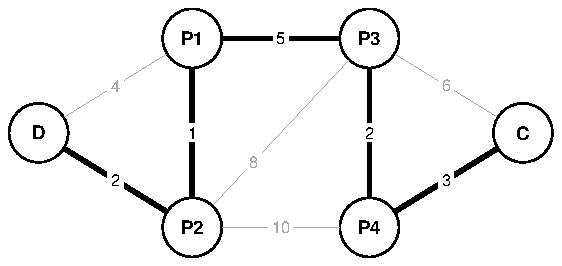
\includegraphics[width=0.75\textwidth]{imagens/grafo-coleta.pdf}
  \caption*{Fonte: Elaborada pela autora (2026).}
\end{figure}

A figura foi inserida com o código abaixo. A legenda vem antes da imagem,
porque o Manual pede a identificação na parte superior, com o número, um
travessão e o título sem ponto final (p. 16). Abaixo da imagem vai a fonte,
obrigatória mesmo quando a figura é da própria autora (p. 17). A classe deixa
a legenda e a fonte em tamanho 10 e espaço simples.

\begin{lstlisting}[language={[LaTeX]TeX}, numbers=none]
\begin{figure}[htbp]
  \caption{Grafo de um setor de coleta, com a rota mínima de D até C em destaque}
  \label{fig:grafo}
  \centering
  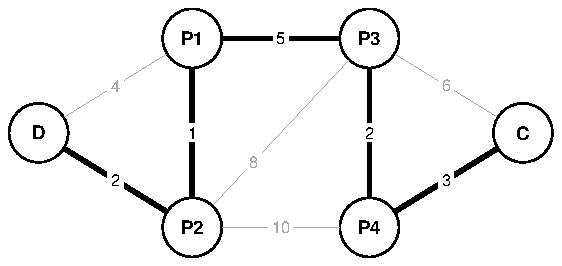
\includegraphics[width=0.75\textwidth]{imagens/grafo-coleta.pdf}
  \caption*{Fonte: Elaborada pela autora (2026).}
\end{figure}
\end{lstlisting}

O caminho da imagem é relativo à pasta onde o documento é compilado, que é a
raiz do repositório. Se a figura vier de outra obra, a fonte traz a citação,
por exemplo \verb|\caption*{Fonte: \citet{Cormen:2022:IA}.}|, e a obra entra nas
referências (Manual, p. 17).

\section{Implementação}

O protótipo foi escrito em Python, com a fila de prioridade do módulo
\texttt{heapq}. A Figura~\ref{fig:codigo} mostra a função principal, aplicada
ao grafo da Figura~\ref{fig:grafo}. Ao ser executada, ela imprime a distância
13 e o caminho D, P2, P1, P3, P4, C.

\begin{figure}[htbp]
  \caption{Implementação do algoritmo de Dijkstra em Python}
  \label{fig:codigo}
\begin{lstlisting}[language=Python]
import heapq

def dijkstra(grafo, origem):
    dist = {v: float("inf") for v in grafo}
    anterior = {v: None for v in grafo}
    dist[origem] = 0
    fila = [(0, origem)]
    while fila:
        d_u, u = heapq.heappop(fila)
        if d_u > dist[u]:
            continue  # entrada antiga da fila
        for v, peso in grafo[u].items():
            if dist[u] + peso < dist[v]:
                dist[v] = dist[u] + peso
                anterior[v] = u
                heapq.heappush(fila, (dist[v], v))
    return dist, anterior

grafo = {
    "D":  {"P1": 4, "P2": 2},
    "P1": {"D": 4, "P2": 1, "P3": 5},
    "P2": {"D": 2, "P1": 1, "P3": 8, "P4": 10},
    "P3": {"P1": 5, "P2": 8, "P4": 2, "C": 6},
    "P4": {"P2": 10, "P3": 2, "C": 3},
    "C":  {"P3": 6, "P4": 3},
}
dist, anterior = dijkstra(grafo, "D")
caminho, v = [], "C"
while v is not None:
    caminho.append(v)
    v = anterior[v]
print(dist["C"], caminho[::-1])  # 13 ['D', 'P2', 'P1', 'P3', 'P4', 'C']
\end{lstlisting}
  \caption*{Fonte: Elaborada pela autora (2026).}
\end{figure}

A listagem foi feita com o ambiente \texttt{lstlisting}, do pacote
\texttt{listings}, dentro de um ambiente \texttt{figure}: assim como o
pseudocódigo, o código-fonte é uma ilustração e recebe o nome de Figura. O
estilo das listagens (fonte, numeração de linhas, moldura e acentos) está no
comando \verb|\lstset| do preâmbulo.

\section{Uso de inteligência artificial}

Na elaboração deste trabalho, utilizou-se a ferramenta de inteligência
artificial generativa [nome e versão da ferramenta], entre [mês/ano] e
[mês/ano], exclusivamente para [finalidades, por exemplo: revisão ortográfica
e tradução do resumo para a língua inglesa]. A ferramenta não foi utilizada
para gerar dados, análises, interpretações ou conclusões. Todo o conteúdo
sugerido foi revisado, editado e validado pela autora, que assume integral
responsabilidade pelo texto final, pela exatidão das informações e pela
autoria intelectual do trabalho.

O parágrafo acima é o modelo de declaração da pasta \texttt{instruções/} do
repositório. Se usar uma ferramenta desse tipo, preencha os trechos entre
colchetes; se não usar, apague a seção.

%==============================================================================
\chapter{Resultados}
\label{cap:resultados}
%==============================================================================

A Tabela~\ref{tab:resultados} compara a distância das rotas praticadas com a
das rotas calculadas nos quatro setores.

\begin{table}[htbp]
  \caption{Distância percorrida por setor, em quilômetros}
  \label{tab:resultados}
  \centering
  \begin{tabular}{lrrr}
    \hline
    Setor & Rota praticada & Rota calculada & Redução (\%) \\
    \hline
    1 -- Centro      & 18,6 & 15,2 & 18,3 \\
    2 -- Fragata     & 22,4 & 19,8 & 11,6 \\
    3 -- Três Vendas & 25,1 & 22,0 & 12,4 \\
    4 -- Areal       & 20,3 & 17,9 & 11,8 \\
    \hline
    Média            & 21,6 & 18,7 & 13,5 \\
    \hline
  \end{tabular}
  \caption*{Fonte: Elaborada pela autora (2026), com dados fictícios para fins de exemplo.}
\end{table}

A tabela segue a padronização do Instituto Brasileiro de Geografia e
Estatística (\pdftooltip{IBGE}{Instituto Brasileiro de Geografia e Estatística}),
indicada pelo Manual (p. 17): traços
horizontais no cabeçalho e no fim, sem traços verticais e sem fechar as
laterais. O título vai em cima e a fonte embaixo, como nas figuras. Valores
numéricos ficam alinhados à direita (\texttt{r} na especificação das
colunas).

\section{Análise por setor}

O setor 1 teve a maior redução. É o setor com mais ruas de mão única, e a rota
praticada fazia retornos longos que o algoritmo evitou.

\subsection{Setores com traçado regular}

Esta é uma seção terciária. A classe numera as seções até o quinto nível,
como pede o Manual (p. 70), e todas aparecem no sumário em negrito.

\subsubsection{Setor 1 -- Centro}

Esta é uma seção quaternária, criada com \verb|\subsubsection|.

\paragraph{Trecho entre a garagem e o primeiro ponto}

Esta é uma seção quinária, criada com \verb|\paragraph|. Não use níveis abaixo
deste: o Manual limita a numeração progressiva à seção quinária.

%==============================================================================
\chapter{Considerações finais}
\label{cap:consideracoes}
%==============================================================================

O algoritmo de Dijkstra reduziu a distância percorrida nos quatro setores
estudados, com redução média de 13,5\% (Tabela~\ref{tab:resultados}). O ganho
foi maior onde as ruas de mão única tornam a rota intuitiva mais longa. O modelo ainda
ignora o tempo de parada em cada ponto e as janelas de horário, que ficam como
trabalho futuro, com variações do problema de roteamento de veículos.

Os apêndices trazem material produzido pela autora: o Apêndice~\ref{apx:dados}
lista os dados do grafo, e o Apêndice~\ref{apx:referencias} mostra como
cadastrar cada tipo de referência. O Anexo~\ref{anx:meses} reproduz material de
outra autoria.

%------------------------------------------------------------------------------
% Referências: estilo abnt.bst e base bibliografia.bib, ambos na raiz.
%------------------------------------------------------------------------------
\bibliographystyle{abnt}
\bibliography{bibliografia}

%------------------------------------------------------------------------------
% Apêndices: material elaborado pela própria autora (Manual, p. 23).
% \apendices cria a folha de abertura; cada \chapter vira "Apêndice A – ...".
%------------------------------------------------------------------------------
\apendices

\chapter{Dados do grafo de exemplo}
\label{apx:dados}

O grafo da Figura~\ref{fig:grafo} tem seis vértices e nove arestas. Os pesos
são as distâncias em quilômetros usadas no código da
Figura~\ref{fig:codigo}: D--P1, 4; D--P2, 2; P1--P2, 1; P1--P3, 5; P2--P3, 8;
P2--P4, 10; P3--P4, 2; P3--C, 6; P4--C, 3. As distâncias mínimas a partir de
D, calculadas pelo algoritmo, são: P2, 2; P1, 3; P3, 8; P4, 10; C, 13.

Apêndices e anexos são numerados com letras e citados no texto pelo nome
seguido da letra, como Apêndice~\ref{apx:referencias} (Manual, p. 23).

\chapter{Exemplos de referências por tipo de documento}
\label{apx:referencias}

Este apêndice cita todas as entradas do arquivo \texttt{bibliografia.bib},
para que a lista de referências deste exemplo mostre como o estilo
\texttt{abnt.bst} formata cada tipo. O arquivo traz, acima de cada entrada, um
comentário explicando quando usar aquele tipo.

Artigos de periódico usam o tipo \texttt{article}:
\citet{Turing:1937:OCN}, \citet{Turing:1950:CMI}, \citet{Shannon:1948:MTC},
\citet{Dijkstra:1959:NTP}, \citet{Dijkstra:1968:GTS}, \citet{Hoare:1969:ABC},
\citet{Codd:1970:RMD}, \citet{Lamport:1978:TCO},
\citet{Dantzig:1959:TDP} e \citet{Solomon:1987:AVR}.

Trabalhos acadêmicos usam \texttt{mastersthesis}, para TCC e dissertação, como
\citet{Cruz:2015:FCS} e \citet{Shannon:1940:SAR}, e \texttt{phdthesis}, para
tese, como \citet{Turing:1938:SLO}. Relatórios técnicos usam
\texttt{techreport}: \citet{vonNeumann:1945:FDR} e \citet{Postel:1981:IP}.

Livros usam \texttt{book}: \citet{vonNeumann:1966:TSR},
\citet{Knuth:1997:ACP}, \citet{Cormen:2022:IA}, \citet{Brooks:1975:MMM},
\citet{Abelson:1996:SIC} e \citet{Moore:1979:MAI}. Um capítulo de livro do
mesmo autor usa \texttt{inbook} \citep{Knuth:1997:IS}; um capítulo de livro
organizado por outra pessoa, \texttt{incollection}
\citep{vonNeumann:1951:GLT}.

Trabalhos publicados em anais de eventos usam \texttt{inproceedings}
\citep{Cook:1971:CTP}; os anais no todo, \texttt{proceedings}
\citep{ACM:1971:STOC}. Normas técnicas usam \texttt{manual}
\citep{ABNT:2018:NBR6023}. Folhetos usam \texttt{booklet}
\citep{Zorzo:2017:RFC}, e documentos não publicados, \texttt{unpublished}
\citep{Dijkstra:1988:CRT}.

Os demais documentos usam \texttt{misc}: preprint
\citep{Vaswani:2017:AIA}, página da web \citep{ACM:2026:TA}, programa de
computador \citep{Aguiar:2026:TEX}, legislação \citep{Brasil:2015:LBI} e
conjunto de dados \citep{Fisher:1936:IRI}.

%------------------------------------------------------------------------------
% Anexos: material de outra autoria (Manual, p. 23-24).
%------------------------------------------------------------------------------
\anexos

\chapter{Abreviatura dos meses em português}
\label{anx:meses}

\begin{table}[htbp]
  \caption{Abreviatura dos meses em português}
  \centering
  \begin{tabular}{llll}
    \hline
    Mês & Abreviatura & Mês & Abreviatura \\
    \hline
    janeiro   & jan.  & julho    & jul. \\
    fevereiro & fev.  & agosto   & ago. \\
    março     & mar.  & setembro & set. \\
    abril     & abr.  & outubro  & out. \\
    maio      & maio  & novembro & nov. \\
    junho     & jun.  & dezembro & dez. \\
    \hline
  \end{tabular}
  \caption*{Fonte: \citet{ABNT:2018:NBR6023}.}
\end{table}

\end{document}
